\documentclass[11pt, letterpaper]{article}
\input{/home/hyperion/.config/LatexHub/preambles/base.tex}
\input{/home/hyperion/.config/LatexHub/preambles/tikz.tex}
\input{/home/hyperion/.config/LatexHub/preambles/diagrams.tex}
\input{/home/hyperion/.config/LatexHub/preambles/macros-cat-theory.tex}
\input{/home/hyperion/.config/LatexHub/preambles/macros-algebra.tex}
\input{/home/hyperion/.config/LatexHub/preambles/basic-theorems-section.tex}
\input{/home/hyperion/.config/LatexHub/preambles/refs-basic.tex}
\input{/home/hyperion/.config/LatexHub/preambles/physics.tex}
\input{/home/hyperion/.config/LatexHub/preambles/code.tex}
\usepackage{titlepageBU}
\theoremstyle{plain}
\newtheorem{problem}{Problem}[section]


\usepackage{titlesec}
\titleformat{\section}{\normalfont\Large\bfseries}{}{0em}{}

\usepackage{titlepageBU}
\title{Midterm 1}
\begin{document}
\makeproblem
\part{Quickies}
\section{Q1 Traveling Gaussian wavepacket}

(a) We just read the distance between peaks off of the graph. It appears to be about $1\,\mathrm{nm} $.

(b) A wavepacket moving to the left is of the form $e^{-ik_0x} $, $k_0>0$. This tells us that the real plot should be a cosine centered at 0, and the imaginary plot should be a sin centered at 0. The fact that $k_0>0$ tells us that the real part starts positive and decreases (since cosine is even), and the imaginary part starts at 0 and decreases as $x$ increases, increasing as $x$ decreases. This is exactly the observed behavior.

The group velocity $v_g=\hbar k_0/m_e$. Since $k_0=2\pi /\lambda $ for $\lambda $ the wavelength, we have $k_0=2\pi \,\mathrm{nm} ^{-1} $. Plugging in values yields $v_g \approx -7.27 \cdot 10^5 \,\mathrm{m} /\mathrm{s} $. The phase velocity $v_p=\frac{1}{2} v_g \approx -3.64\cdot 10^5\,\mathrm{m} /\mathrm{s} $.

(c) Standard deviation of a Gaussian with initial standard deviation $\sigma _0$ has
\[
	\sigma _x^2=\sigma _0^2 \left( 1+\left( \frac{\hbar t}{2m\sigma _0^2}  \right) ^2 \right) 
.\]
Set $\sigma _x^2=2\sigma _0^2$. Solving gives
\[
	t_{\mathrm{nat} } =\tau =\frac{2m\sigma _0^2}{\hbar} 
.\]
The halfway point at the Gaussian appears around 1 nm, and for Gaussians it occurs at approximately $2.3 \sigma _0$. Solving gives $\sigma _0 \approx 0.85\,\mathrm{nm} $. Plugging in the numbers gives
\[
	\tau \approx 2\frac{\left( 9.1\cdot 10^{-31} \,\mathrm{kg}  \right) \left( \frac{10^{-9} \,\mathrm{nm} }{2.355}  \right) ^2}{1.054\cdot 10^{-34} \,\mathrm{J} \cdot \mathrm{s} } \approx 3\cdot 10^{-15} \,\mathrm{s} 
.\]

\section{Q2 Natural units}

(i) $1\,\mathrm{mW} =10^{-3} \frac{\mathrm{J} }{\mathrm{s} } $, $1\,\mathrm{mm} ^2=10^{-6} \,\mathrm{m} ^2$. Thus the intensity is $10^3\,\mathrm{W} /\mathrm{m} ^2$. Now we just use the conversions into natural units
\[
	1\,\mathrm{J} =6.242\cdot 10^{18} \,\mathrm{eV} ,
\]
\[
	\hbar c=1.97\cdot 10^{-7} \,\mathrm{eV} \cdot \mathrm{m} 
.\]
We have
\[
	1\mathrm{m} =\frac{1}{1.97} \,\mathrm{eV} ^{-1} =5.07\cdot 10^{6} \,\mathrm{eV} ^{-1} 
.\]
\[
	1\,\mathrm{s} =\frac{1}{c} \,\mathrm{m} \approx 3\cdot 10^8\,\mathrm{m} \implies 1\,\mathrm{s} =1.52\cdot 10^{15} \,\mathrm{eV} ^{-1} 
.\]
Plugging in gives
\[
	I=10^3\left( 6.242\cdot 10^{18} \,\mathrm{eV}  \right) \left( 1.52\cdot 10^{15} \,\mathrm{eV} ^{-1}  \right) ^{-1} \left( 5.07\cdot 10^6\,\mathrm{eV} ^{-1}  \right) ^{-2} \approx 2\cdot 10^{-7} \,\mathrm{eV} ^4
.\]

(ii,iii) I don't know, and I feel using a lifeline without putting down a coherent answer would be a very cheap cop-out.
\section{Q3 Two level system, Bloch sphere}
(a) The matrix representation of $\mathbf{H} $ is given by
\[
	-\frac{\Delta }{2} \begin{pmatrix}
	1 & 0 \\
	0 & -1
	\end{pmatrix}+\frac{1}{2} \left( \begin{pmatrix}
	0 & \gamma _+ \\
	\gamma _+ & 0
	\end{pmatrix}+i\begin{pmatrix}
	0 & -i \gamma _+ \\
	i\gamma _+ & 0
	\end{pmatrix}+\begin{pmatrix}
	0 & \gamma _- \\
	\gamma _- & 0
	\end{pmatrix}+i\begin{pmatrix}
	0 & i\gamma _- \\
	-i\gamma _- & 0
	\end{pmatrix} \right)
\]
\[
	=\frac{1}{2} \begin{pmatrix}
	-\Delta  & \gamma _++\gamma _++\gamma _- -\gamma _- \\
	\gamma _+-\gamma _++\gamma _- +\gamma _- & \Delta 
	\end{pmatrix}=\begin{pmatrix}
	-\frac{\Delta }{2}   & \gamma _+ \\
	\gamma _- & \frac{\Delta }{2} 
	\end{pmatrix}
.\]
For $\mathbf{H} $ to be Hermitian, we must have $\mathbf{H} ^\dagger = \mathbf{H} $. This gives the equality
\[
	\begin{pmatrix}
	-\frac{\Delta }{2}  & \gamma _+ \\
	\gamma _- & \frac{\Delta }{2} 
	\end{pmatrix}=\begin{pmatrix}
	-\frac{\Delta }{2}  & \gamma _-^* \\
	\gamma _+^* & \frac{\Delta }{2} 
	\end{pmatrix}
.\]
Here we have used the fact that $\Delta $ is real. Therefore, $\gamma _+=\gamma _-^*$, and vice versa.

(b) I'm unsure how HW 3.3 is helpful, but in HW 3.2 we solved for the eigenvectors in the $\ket{0},\ket{1}$ basis. Since we are allowed to consult solutions to \emph{any} homework problems, this is still fair game. Write $\ket{\psi _0},\ket{\psi _1}$ for the eigenstates. We found
\[
	\ket{\psi _0} = \cos \frac{\theta }{2} \ket{0} + e^{i\chi }\sin \frac{\theta }{2}  \ket{1}
,\]
\[
	\ket{\psi _1} = \sin \frac{\theta }{2} \ket{0} - e^{i\chi } \cos \frac{\theta }{2} \ket{1}
.\]
Of course, HW 3.2 used a different Hamiltonian
\[
	\mathbf{H} ' = \begin{pmatrix}
	\varepsilon _0 & \gamma e^{-i\chi }  \\
	\gamma e^{i\chi }  & \varepsilon _1
	\end{pmatrix},\qquad \varepsilon _0<\varepsilon _1,\,\, \varepsilon _0,\varepsilon _1,\gamma,\chi  \in\mathbb{R} ,\,\, 0\leq \gamma ,\chi 
.\]
Most of the assumptions are necessary, since $\theta $ was defined as the unique angle along $[0,\pi ]$ such that
\[
	\tan \theta =\frac{2\gamma }{\varepsilon _0-\varepsilon _1} 
.\]
Since $\Delta >0$, we have $-\Delta/2 <\Delta/2 $, so the diagonal elements are of the same form as this Hamiltonian. It suffices to show that the off-diagonal elements can be put in the form $\gamma e^{\pm i\chi } $. The eigenstates of the given Hamiltonian will then be of the same form. Indeed, since $\gamma _\pm,\gamma _\pm^*$ are all complex numbers, the diagonal elements are complex numbers, and thus admit a polar representation
\[
	\gamma _1 e^{-i\chi _1} =\gamma _+,
\]
\[
	\gamma _2 e^{i\chi _2} =\gamma _-
.\]
It suffices to show $\gamma _1=\gamma _2$ and $\chi _1=\chi _2$, since we may always take $\gamma _1,\chi _1\geq 0$.

This follows immediately by the fact that $\gamma _+^*=\gamma _-$:
\[
	\gamma_1 e^{i\chi _1} =\gamma _+^* = \gamma _- = \gamma _2 e^{i\chi _2} 
.\]
Since $\gamma _1,\gamma _2 \geq 0$, computing the norm gives
\[
	\gamma _1=\left| \gamma _1 e^{i\chi _1}  \right|=\left| \gamma _2e^{i\chi _2}  \right| =\gamma _2
.\]
Therefore, $\gamma _1=\gamma _2$. Dividing out then gives $e^{i\chi _1} =e^{i\chi _2} $. Taking the natural logarithm yields $i\chi _1=i\chi _2$ (alternatively, appeal to bijectivity of exp on $\mathbb{C} $). It follows that $\chi _1=\chi _2$. Therefore, there exist $\gamma ,\chi $ such that the given Hamiltonian is of the same form as the one in HW 3, and our eigenstates are the exact same. The angle $\theta $ for this Hamiltonian is given by
\[
	\tan \theta =\frac{2\gamma }{\frac{-\Delta -\Delta }{2}} =-\frac{2\gamma }{\Delta } 
.\]

(c) We have
\[
	\tan \theta =-\frac{2\gamma }{2\gamma } =-1
.\]
Since we choose $0\leq \theta \leq \pi $, we have $\theta =3\pi /4$. Since $\gamma _+,\gamma _-\in\mathbb{R} $, we have $\chi =0$. This yields
\[
	\ket{\psi _0}= \cos \frac{3\pi }{8} \ket{0}+ \sin \frac{3\pi }{8} \ket{1},
\]
\[
	\ket{\psi _1}=\sin \frac{3\pi }{8} \ket{0}- \cos \frac{3\pi }{8} \ket{1}
.\]
I chose to plot these with Qiskit.
\begin{lstlisting}[language=Python]
import numpy as np
from qiskit.visualization import plot_bloch_multivector
from qiskit.quantum_info import Statevector

theta = np.pi * 3 / 8
psi0 = Statevector([np.cos(theta), np.sin(theta)])
psi1 = Statevector([np.sin(theta), -1 * np.cos(theta)])
 
plot_bloch_multivector(psi0)
\end{lstlisting}
\begin{figure}[ht]
	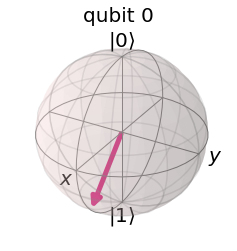
\includegraphics[scale=0.7]{block-1.png}
	\centering
\end{figure}
\begin{lstlisting}[language=Python]
plot_bloch_multivector(psi1)
\end{lstlisting}
\begin{figure}[ht]
	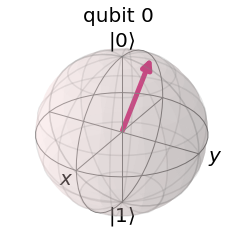
\includegraphics[scale=0.7]{block-2.png}
	\centering
\end{figure}

\section{Q4 Equation of motion and a proof of entanglement}

(a) We take the time derivative of $\rho $ and apply the Schr\"odinger equation.

\[
	\frac{\partial \rho }{\partial t} =\frac{\partial }{\partial t} \ket{\Psi (t)}\bra{\Psi (t)}=\left( \frac{\partial \ket{\Psi (t)}}{\partial t}  \right) \bra{\Psi (t)} + \ket{\Psi (t)}\frac{\partial \bra{\Psi (t)}}{\partial t} 
.\]
The Schr\"odinger equation gives
\[
	\frac{\partial \ket{\Psi (t)}}{\partial t} =-\frac{i}{\hbar} \mathbf{H} \ket{\Psi (t)}
.\]
To figure out the equation for $\bra{\Psi (t)}$, we use the fact that $\mathbf{H} $ is Hermitian and take the conjugate of both sides:
\[
	-i\hbar\frac{\partial \bra{\Psi (t)}}{\partial t} =\left(i\hbar \frac{\partial \ket{\Psi (t)}}{\partial t}  \right) ^\dagger = \left( \mathbf{H} \ket{\Psi (t)} \right) ^\dagger = \bra{\Psi (t)}\mathbf{H} 
.\]
Plugging this in yields
\[
	\frac{\partial \rho }{\partial t} =\left( -\frac{i}{\hbar} \mathbf{H} \ket{\Psi (t)} \right) \bra{\Psi (t)}+\ket{\Psi (t)}\left( \frac{i}{\hbar} \bra{\Psi (t)}\mathbf{H}  \right) =\frac{i}{\hbar}\left( \ket{\Psi (t)}\bra{\Psi (t)}\mathbf{H} -\mathbf{H} \ket{\Psi (t)}\bra{\Psi (t)} \right)
.\]
This gives us the equation of motion
\[
	\frac{\partial \rho }{\partial t} =\frac{i}{\hbar} \left( \rho (t)\mathbf{H} -\mathbf{H} \rho (t) \right) =\frac{i}{\hbar} \left[ \rho (t),\mathbf{H}  \right] 
.\]

(b) The proof is explicitly given in the October 2nd lecture notes. We follow the proof given there. We must show that $\ket{\Psi _3}$ cannot be written as a pure tensor $\ket{\psi _A}\otimes \ket{\psi _B}$. Suppose for contradiction that kets $\ket{\psi _A},\ket{\psi _B}$ exist such that $\ket{\Psi _3}=\ket{\psi _A}\otimes \ket{\psi _B}$. Since $\ket{0},\ket{1}$ forms a basis for the Hilbert space $\mathcal{H}_{A\text{ or } B} $ (where $\ket{\Psi _3}\in \mathcal{H}_A \otimes \mathcal{H}_B $), there are complex coefficients $a_0,a_1,b_0,b_1\in\mathbb{C} $ such that
\[
	\ket{\psi _A}=a_0\ket{0_A}+a_1\ket{1_A},\qquad \ket{\psi _B}=b_0\ket{0_B}+b_1\ket{1_B}
.\]
This gives us
\[
	\ket{\Psi _3}=\left( a_0\ket{0_A}+a_1\ket{1_A} \right) \otimes \left( b_0\ket{0_B}+b_1\ket{1_B} \right) 
.\]
Bilinearity of tensor implies that this distributes as
\[
	\ket{\Psi _3}=a_0b_0\ket{0_A}\otimes \ket{0_B}+a_0b_1\ket{0_A}\otimes \ket{1_B}+a_1b_0\ket{1_A}\otimes \ket{0_B}+a_1b_1\ket{1_A}p\otimes \ket{1_B}
.\]
This must equal the original state
\[
	\ket{\Psi _3}=\frac{1}{\sqrt{2} } \ket{0_A}\otimes \ket{0_B}-\frac{1}{\sqrt{2} } \ket{1_A}\otimes \ket{1_B}
.\]
We then obtain from uniqueness of basis representations that
\[
	a_0b_0=\frac{1}{\sqrt{2} } ,\qquad a_1b_1=-\frac{1}{\sqrt{2} } ,\qquad a_0b_1=a_1b_0=0
.\]
The lecture notes finish the proof by considering normalization, but we already have an easier contradiction. Because $\mathbb{C} $ has no zero divisors, $a_0b_1=0$ if and only if at least one of $a_0,b_1$ is 0. If $a_0=0$ then $a_0b_0=0 \neq 1/\sqrt{2} $, a contradiction. If $b_1=0$ then $a_1b_1=0 \neq -1/\sqrt{2} $, another contradiction. Therefore, we cannot have $a_0$ or $b_1$ equal to 0, giving us our contradiction.

\section{Q5 Dyson series and the Magnus expansion}

(a) We are given the second order approximation
\[
	U_I(t,t_0)=1+\frac{i}{\hbar} \int_{t_0}^{t} V_I(t_1) \,\mathrm{d} t_1-\frac{1}{2\hbar^2} \int_{t_0}^{t}\int_{t_0}^{t_2} [V_I(t_2),V_I(t_1)] \,\mathrm{d} t_1 \mathrm{d} t_2
.\]
Recall that in the interaction picture, the equation of motion is
\[
	i\hbar \frac{\partial U_I}{\partial t} =V_IU_I
.\]
We differentiate each term in the expansion separately. We start with the first integral and apply the fundamental theorem of calculus:
\[
	\frac{\partial }{\partial t} \frac{i}{\hbar} \int_{t_0}^{t} V_I(t_1) \,\mathrm{d} t_1=\frac{i}{\hbar} V_I(t)
.\]
For the second integral,
\[
	-\frac{1}{2\hbar^2} \frac{\partial }{\partial t} \int_{t_0}^{t}\int_{t_0}^{t_2} \left[ V_I(t_2),V_I(t_1) \right]  \,\mathrm{d} t_1 \mathrm{d} t_2=-\frac{1}{2\hbar^2} \int_{t_0}^{t} \left[ V_I(t),V_I(t_1) \right]  \,\mathrm{d} t_1
.\]
We obtain
\[
	\frac{\partial U_I}{\partial t} =\frac{i}{\hbar} V_I(t)-\frac{1}{2\hbar^2} \int_{t_0}^{t} [V_I(t),V_I(t_1)] \,\mathrm{d} t_1=\frac{i}{\hbar} V_I(t)-\frac{1}{2\hbar^2} \int_{t_0}^{t} V_I(t)V_I(t_1) \,\mathrm{d} t_1-\frac{1}{2\hbar^2} \int_{t_0}^{t} V_I(t_1)V_I(t) \,\mathrm{d} t_1
\]
\[
	=\frac{i}{\hbar} V_I(t)-\frac{V_I(t)}{2\hbar^2} \int_{t_0}^{t} V_I(t_1) \,\mathrm{d} t_1 - \frac{1}{2\hbar^2} \left( \int_{t_0}^{t} V_I(t_1) \,\mathrm{d} t_1 \right) V_I(t)
.\]
We now check both sides of the equation of motion. For the left, we multiply through by $i\hbar$ to obtain
\[
	V_I(t)-\frac{i}{2\hbar} V_I(t)\int_{t_0}^{t} V_I(t_1) \,\mathrm{d} t_1-\frac{i}{2\hbar} \left( \int_{t_0}^{t} V_I(t_1) \,\mathrm{d} t_1 \right) V_I(t)
.\]
For the right, we compute $V_I(t)U_I(t,t_0)$:
\begin{align*}
	V_IU_I&=V_I(t)\left( 1+\frac{i}{\hbar} \int_{t_0}^{t} V_I(t_1) \,\mathrm{d} t_1-\frac{1}{2\hbar^2} \int_{t_0}^{t}\int_{t_0}^{t_2} \left[ V_I(t_2),V_I(t_1) \right]  \,\mathrm{d} t_1 \mathrm{d} t_2 \right)\\
	      &=V_I(t)+\frac{i}{\hbar}V_I(t)\int_{t_0}^{t} V_I(t_1) \,\mathrm{d} t_1-\frac{1}{2\hbar^2} V_I(t) \int_{t_0}^{t}\int_{t_0}^{t_2} \left[ V_I(t_2),V_I(t_1) \right]  \,\mathrm{d} t_1 \mathrm{d} t_2 \\
	      &=V_I(t)+\frac{i}{\hbar} V_I(t)\int_{t_0}^{t} V_I(t_1) \,\mathrm{d} t_1 - \frac{1}{2\hbar^2} V_I(t)\int_{t_0}^{t}\int_{t_0}^{t_2} V_I(t_2)V_I(t_1) \,\mathrm{d} t_1 \mathrm{d} t_2\\
	      &\quad-\frac{1}{2\hbar^2} V_I(t)\int_{t_0}^{t}\int_{t_0}^{t_2} V_I(t_1)V_I(t_2) \,\mathrm{d} t_1 \mathrm{d} t_2
.\end{align*}
Since we are only concerned with equality up to second order, we drop the higher order terms, obtaining (in the second order approximation)
\[
	V_I U_I = V_I(t)+\frac{i}{\hbar}V_I(t) \int_{t_0}^{t} V_I(t_1) \,\mathrm{d} t_1
.\]
This would be equal to the LHS if $V_I(t)$ commuted with $V_I(t_1)$ \emph{and} if the sign on the second term in the original expression was changed. Unfortunately, none of these are true, since if $V_I(t)$ commuted with $V_I(t_1)$ then the commutator would have vanished long ago. I don't know if the problem is wrong or if I am, since I can't find issues with my reasoning.

(b) 
\[
	U_I^\dagger=1-\frac{i}{\hbar} \int_{t_0}^{t} V_I(t_1) \,\mathrm{d} t_1 -\frac{1}{2\hbar^2} \int_{t_0}^{t}\int_{t_0}^{t_2} \left[ V_I(t_1),V_I(t_2) \right]  \,\mathrm{d} t_1 \mathrm{d} t_2
\]
\[
	=1-\frac{i}{\hbar} \int_{t_0}^{t} V_I(t_1) \,\mathrm{d} t_1+\frac{1}{2\hbar^2} \int_{t_0}^{t}\int_{t_0}^{t_2} \left[ V_I(t_2),V_I(t_1) \right]  \,\mathrm{d} t_1 \mathrm{d} t_2
.\]
Here we have used $V_I^\dagger=V_I$. Because dragging the integrals along is annoying, write $I_1$ for the first integral and $I_2$ for the second. Then
\[
	UU^\dagger = \left( 1+\frac{i}{\hbar} I_1-\frac{1}{2\hbar^2} I_2 \right) \left( 1-\frac{i}{\hbar} I_1+\frac{1}{2\hbar^2} I_2 \right) 
\]
\[
	=1+\frac{i}{\hbar} I_1 - \frac{i}{\hbar} I_1-\frac{1}{2\hbar^2} I_2 + \frac{1}{2\hbar^2} I_2 + \frac{i}{2\hbar^3} I_1I_2 + \frac{i}{2\hbar^3} I_2I_1 + \frac{1}{\hbar^2} I_1^2 - \frac{1}{4\hbar^4} I_2^2
.\]
Although we can drop the higher order terms, I see no way to simplify down $I^2_1/\hbar^2$ to 0 using what we have.


\part{Long problems}
\section{L1 Lorentzian pulse in time}

(a) First order time-dependent perturbation theory gives that the coefficient for transmission $\ket{1}\to \ket{0}$ is computed by the integral
\[
	c_{10} (t)=\frac{1}{i\hbar} \int_{t_0}^{t} \bra{0}V(t)\ket{1}e^{it'\frac{\varepsilon _0-\varepsilon _1}{\hbar} }  \,\mathrm{d} t'
.\]
Of course
\[
	\bra{0}V(t)\ket{1}=\frac{\gamma }{1+\left( \frac{t}{\tau }  \right) ^2} 
.\]
Using $t_0\to -\infty $ and $t\to \infty$, we have
\[
	c_{10} (\tau )=\frac{1}{i\hbar} \int_{-\infty }^{\infty } \frac{\gamma }{1+\left( \frac{t'}{\tau }  \right) ^2} \exp \left( \frac{it'(\varepsilon _0-\varepsilon _1)}{\hbar}  \right)  \,\mathrm{d} t'=\frac{\gamma }{i\hbar} \int_{-\infty }^{\infty } \frac{\tau ^2}{\tau ^2+t^{\prime 2} } \exp \left( \frac{it'(\varepsilon _0-\varepsilon _1)}{\hbar}  \right)  \,\mathrm{d} t'
.\]
This is an annyoing integral. Writing $\omega =(\varepsilon _0-\varepsilon _1)/\hbar$, we solve with Mathematica.
\begin{lstlisting}[language=Mathematica]
Integrate[(tau^2 / (t^2 + tau^2)) * Exp[I * omega * t], {t, -Infinity, Infinity},
  Assumptions -> {tau > 0, Element[omega, Reals]}]
\end{lstlisting}
This outputs $\pi \tau e^{-\tau \left| \omega  \right| } $. We thus have
\[
	c_{10} (\tau )=\frac{\gamma \pi \tau }{i\hbar} \exp \left( \frac{\varepsilon _0-\varepsilon _1}{\hbar} \tau  \right) 
.\]
Here we are able to get rid of the absolute value since we know $\varepsilon _0<\varepsilon _1$, so $\left| \omega  \right| =\varepsilon _1-\varepsilon _0$. We can now compute the transition probability:
\[
	P_{1\to 0} (t\to \infty )=\left| \frac{\gamma \pi \tau }{i\hbar} \exp \left( \frac{\varepsilon _0-\varepsilon _1}{\hbar} \tau  \right)  \right| ^2=\frac{\gamma ^2\pi ^2\tau ^2}{\hbar^2} \exp \left( \frac{\varepsilon _0-\varepsilon _1}{\hbar} 2\tau  \right) 
.\]
Here we have used the fact that $\gamma ,\tau ,\hbar,\pi \in\mathbb{R} $ to simplify the norm squared to simply the square, dropping the $i$.

(b) It will be nice to define the dimensionless duration $x=\frac{\tau (\varepsilon _1-\varepsilon _0)}{\hbar} $, and then write
\[
	P_{1\to 0} (t\to \infty )=\frac{\gamma ^2\pi ^2\tau ^2}{\hbar^2} e^{-2x} 
.\]
If we want to plot $x$ on the $x$-axis, we should put the $\tau ^2$ in the prefactor in terms of $x$. Since
\[
	x^2=\frac{\tau ^2\left( \varepsilon _1-\varepsilon _0 \right) ^2}{\hbar^2} ,
.\]
we can define $k=\gamma/(\varepsilon _1-\varepsilon _0)$ and obtain
\[
	P_{1\to 0} (t\to \infty )=k^2\pi ^2x^2e^{-2x} 
.\]
There is now no $\tau $-dependence outside of the $x$-dependence. Additionally, choices of $\gamma /(\varepsilon _1-\varepsilon _0)$ are now choices of the factor $k$.

We want to make sensible choices based on the given conditions. The problem gives $\gamma \ll \varepsilon _1-\varepsilon _0$ which makes $P$ small, which is needed to make first order perturbation theory accurate. We will choose $k$ for some small values: $0.1,0.2,0.3$.

\begin{figure}[ht]
	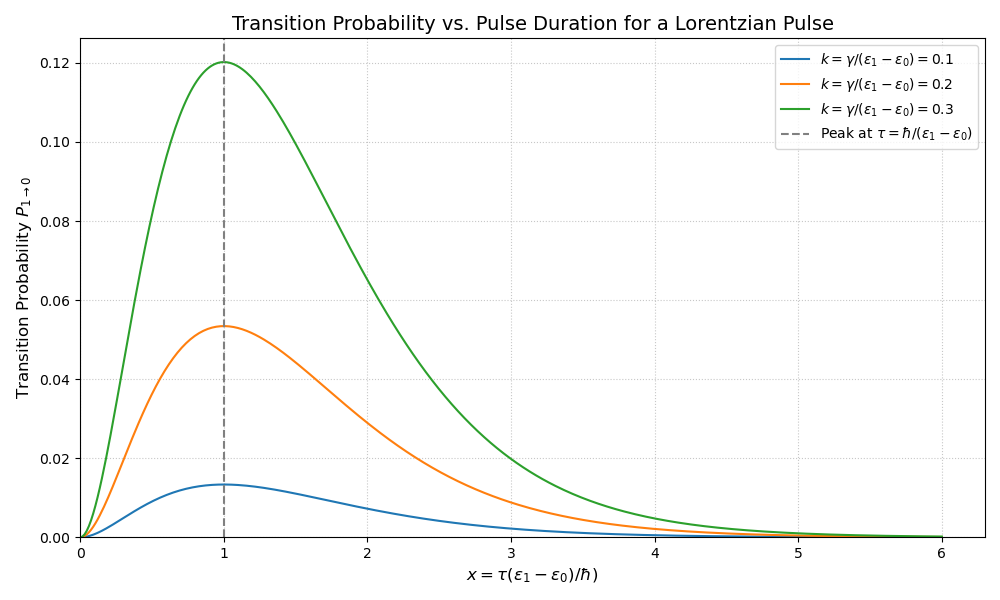
\includegraphics[scale=0.65]{./transition_probability_plot.png}
	\centering
	\caption{Transition probability vs pulse duration for a Lorentzian pulse}
\end{figure}

As $\left| \gamma  \right| \to \varepsilon _1-\varepsilon _0$ the perturbation theory breaks down because $k$ gets close to 1, and the maximum probability actually exceeds 1. Let $\left| \gamma  \right| =\varepsilon _1-\varepsilon _0$, making $k=1$. Taking $\tau =\frac{\hbar}{\varepsilon _1-\varepsilon _0} $ for the maximum, we have $x=1$, and thus
\[
	P_{1\to 0} (t\to \infty )=1^2\pi ^2 1^2 e^{-2} =\frac{\pi ^2}{e^2} 
.\]
Since $\pi >e$, this is greater than 1.

\section{L2 Mach-Zehnder inferometer}
(a) Since the photons are all incident from the top path, the initial state is $\ket{\psi _0}=\ket{0}$. The final state is $B_2M_{12} PB_1\ket{\psi _0}$, where $P$ is the contribution from the phase plate. We can represent $P$ as
\[
	P=\begin{pmatrix}
	1 & 0 \\
	0 & e^{i\phi } 
	\end{pmatrix}
,\]
since relative phase is all that matters. The final state is
\[
	\frac{e^{i\pi /4} }{2} \begin{pmatrix}
	1 & i \\
	i & 1
	\end{pmatrix}\begin{pmatrix}
	1 & 0 \\
	0 & 1
	\end{pmatrix}\begin{pmatrix}
	1 & 0 \\
	0 & e^{i\phi } 
	\end{pmatrix}\begin{pmatrix}
	1 & i \\
	i & 1
	\end{pmatrix}\begin{pmatrix}
	1 \\
	0
	\end{pmatrix}=\frac{e^{i\pi /4} }{2}\begin{pmatrix}
	1-e^{i\phi }  & ie^{i\phi } +i \\
	ie^{i\phi } +i & -1+e^{i\phi } 
	\end{pmatrix}\begin{pmatrix}
	1 \\
	0
	\end{pmatrix}=\frac{e^{i\pi /4} }{2} \begin{pmatrix}
	1-e^{i\phi }  \\
	ie^{i\phi } +i
	\end{pmatrix}
.\]
We need the final state to be $(1,0)$, meaning that $ie^{i\phi } +i=0$. We thus have $e^{i\phi } =-1$, and thus $\phi =n\pi $ for $n$ any odd integer. Therefore, $\phi =\pi $ is a working value.

(b) (i) The bomb is working and intact. If the bomb is a dud, then it has a trivial contribution to the overall probability, and thus the problem reduces to the setup in (a) where there are zero detections in D2. The fact that something was detected in D2 is impossible if the bomb is a dud, so it must be working. A working bomb contributes a matrix
\[
	K=\mathrm{Bomb} =\begin{pmatrix}
	0 & 0 \\
	0 & 1
	\end{pmatrix}
.\]
This is because it absorbs all photons traveling along the top path and none along the bottom. Putting this into the matrix calculation (and taking $\phi =\pi $) yields
\[
	\frac{e^{i\pi /4} }{2} \begin{pmatrix}
	1 & i \\
	i & 1
	\end{pmatrix}\begin{pmatrix}
	1 & 0 \\
	0 & -1
	\end{pmatrix}\begin{pmatrix}
	0 & 0 \\
	0 & 1
	\end{pmatrix}\begin{pmatrix}
	1 & i \\
	i & 1
	\end{pmatrix}\begin{pmatrix}
	1 \\
	0
	\end{pmatrix}=\frac{e^{i\pi /4} }{2} \begin{pmatrix}
	1 \\
	-i
	\end{pmatrix}
.\]
This is \emph{not} normalized, meaning the probability of the photon making it to the end is not 100\%. The probability of a detection in either D2 or D1 is clearly 1/4 due to the factor of 1/2 squaring to 1/4. This means there is a 50\% chance the bomb detonates, a 25\% chance of a detection in D1, and a 25\% chance of a detection in D2. Since we saw a detection in D2, the bomb cannot have exploded.

(ii) We cannot determine whether the bomb is working or not. As seen in (i), there is a 25\% chance of seeing this even if the bomb is working, and a 100\% chance if it is not. We would need to see a D2 detection to know for sure if it is working. It is impossible to tell with 100\% confidence that it is never working, but more data would improve the statistical significance of that result.

(iii) As seen in (i), if the bomb is a dud then we will always see photons in D1, so the bomb cannot be a dud. The only case where a photon is not recieved is if the bomb explodes. Therefore, we got unlucky and detonated the bomb.
\end{document}
